\section{Product perspective}
\subsection{Scenarios}
\textbf{Scenario 1: Path Visualization}\\
Alice is a student who wants to bike from her university to a new gym she has never visited before.
She opens the Best Bike Paths (BBP) application and inputs her current location as the origin and the gym's address as the destination.
The system calculates available routes and displays them on a map. BBP visualizes the paths based on a calculated score ,
which considers both the distance and the quality of the road surface. Alice notices that the shortest path is marked with a lower score because parts of it are tagged as "requires maintenance."
She decides to select a slightly longer but "optimal" path to ensure a smoother ride. She mounts her phone on the bike handlebar and follows the suggested route.

\textbf{Scenario 2: Automated Tracking and Pothole Detection}\\
Bob is an avid cyclist who tracks his daily training sessions. He gets on his bike and starts pedaling without manually interacting with the application.
BBP detects his movement speed and guesses that he is biking, automatically initiating the data acquisition process. As Bob cycles through a park, he accidentally hits a deep pothole.
The application collects data from the smartphone's accelerometer and gyroscope, registering the sudden movement as a potential anomaly.
At the end of the ride, Bob checks his smartphone. The system displays a summary of the trip and asks for verification regarding the anomaly detected in the park.
Bob confirms that there was indeed a pothole, and this information is stored to update the community map.

\textbf{Scenario 3: Scenario 3: Manual Reporting of Road Status}\\
Charlie is cycling home when he encounters a newly repaved bike lane that was previously full of cracks.
He stops safely, opens the BBP application, and chooses to insert information in manual mode. He selects the specific street segment on the map and updates its status to "Optimal."
Since no other conflicting data has been entered recently, BBP immediately considers this path as optimal. Later that day, other users planning a route through that area see the updated status and choose that path for their commute.

\textbf{Scenario 4: Scenario 4: Analyzing Performance and Weather}\\
Diana has just finished a long weekend ride. She opens BBP to review her activity history. The system presents a list of her stored trips. She selects the most recent one to view the details. BBP displays her total distance covered, average speed, and other performance metrics. Additionally, since the system successfully retrieved data from the external meteorological service during her ride, the trip log is enriched with weather information, showing that she maintained a high average speed despite strong headwinds and low temperatures.
\subsection{Class diagram}
\begin{figure}[H]
    \centering
    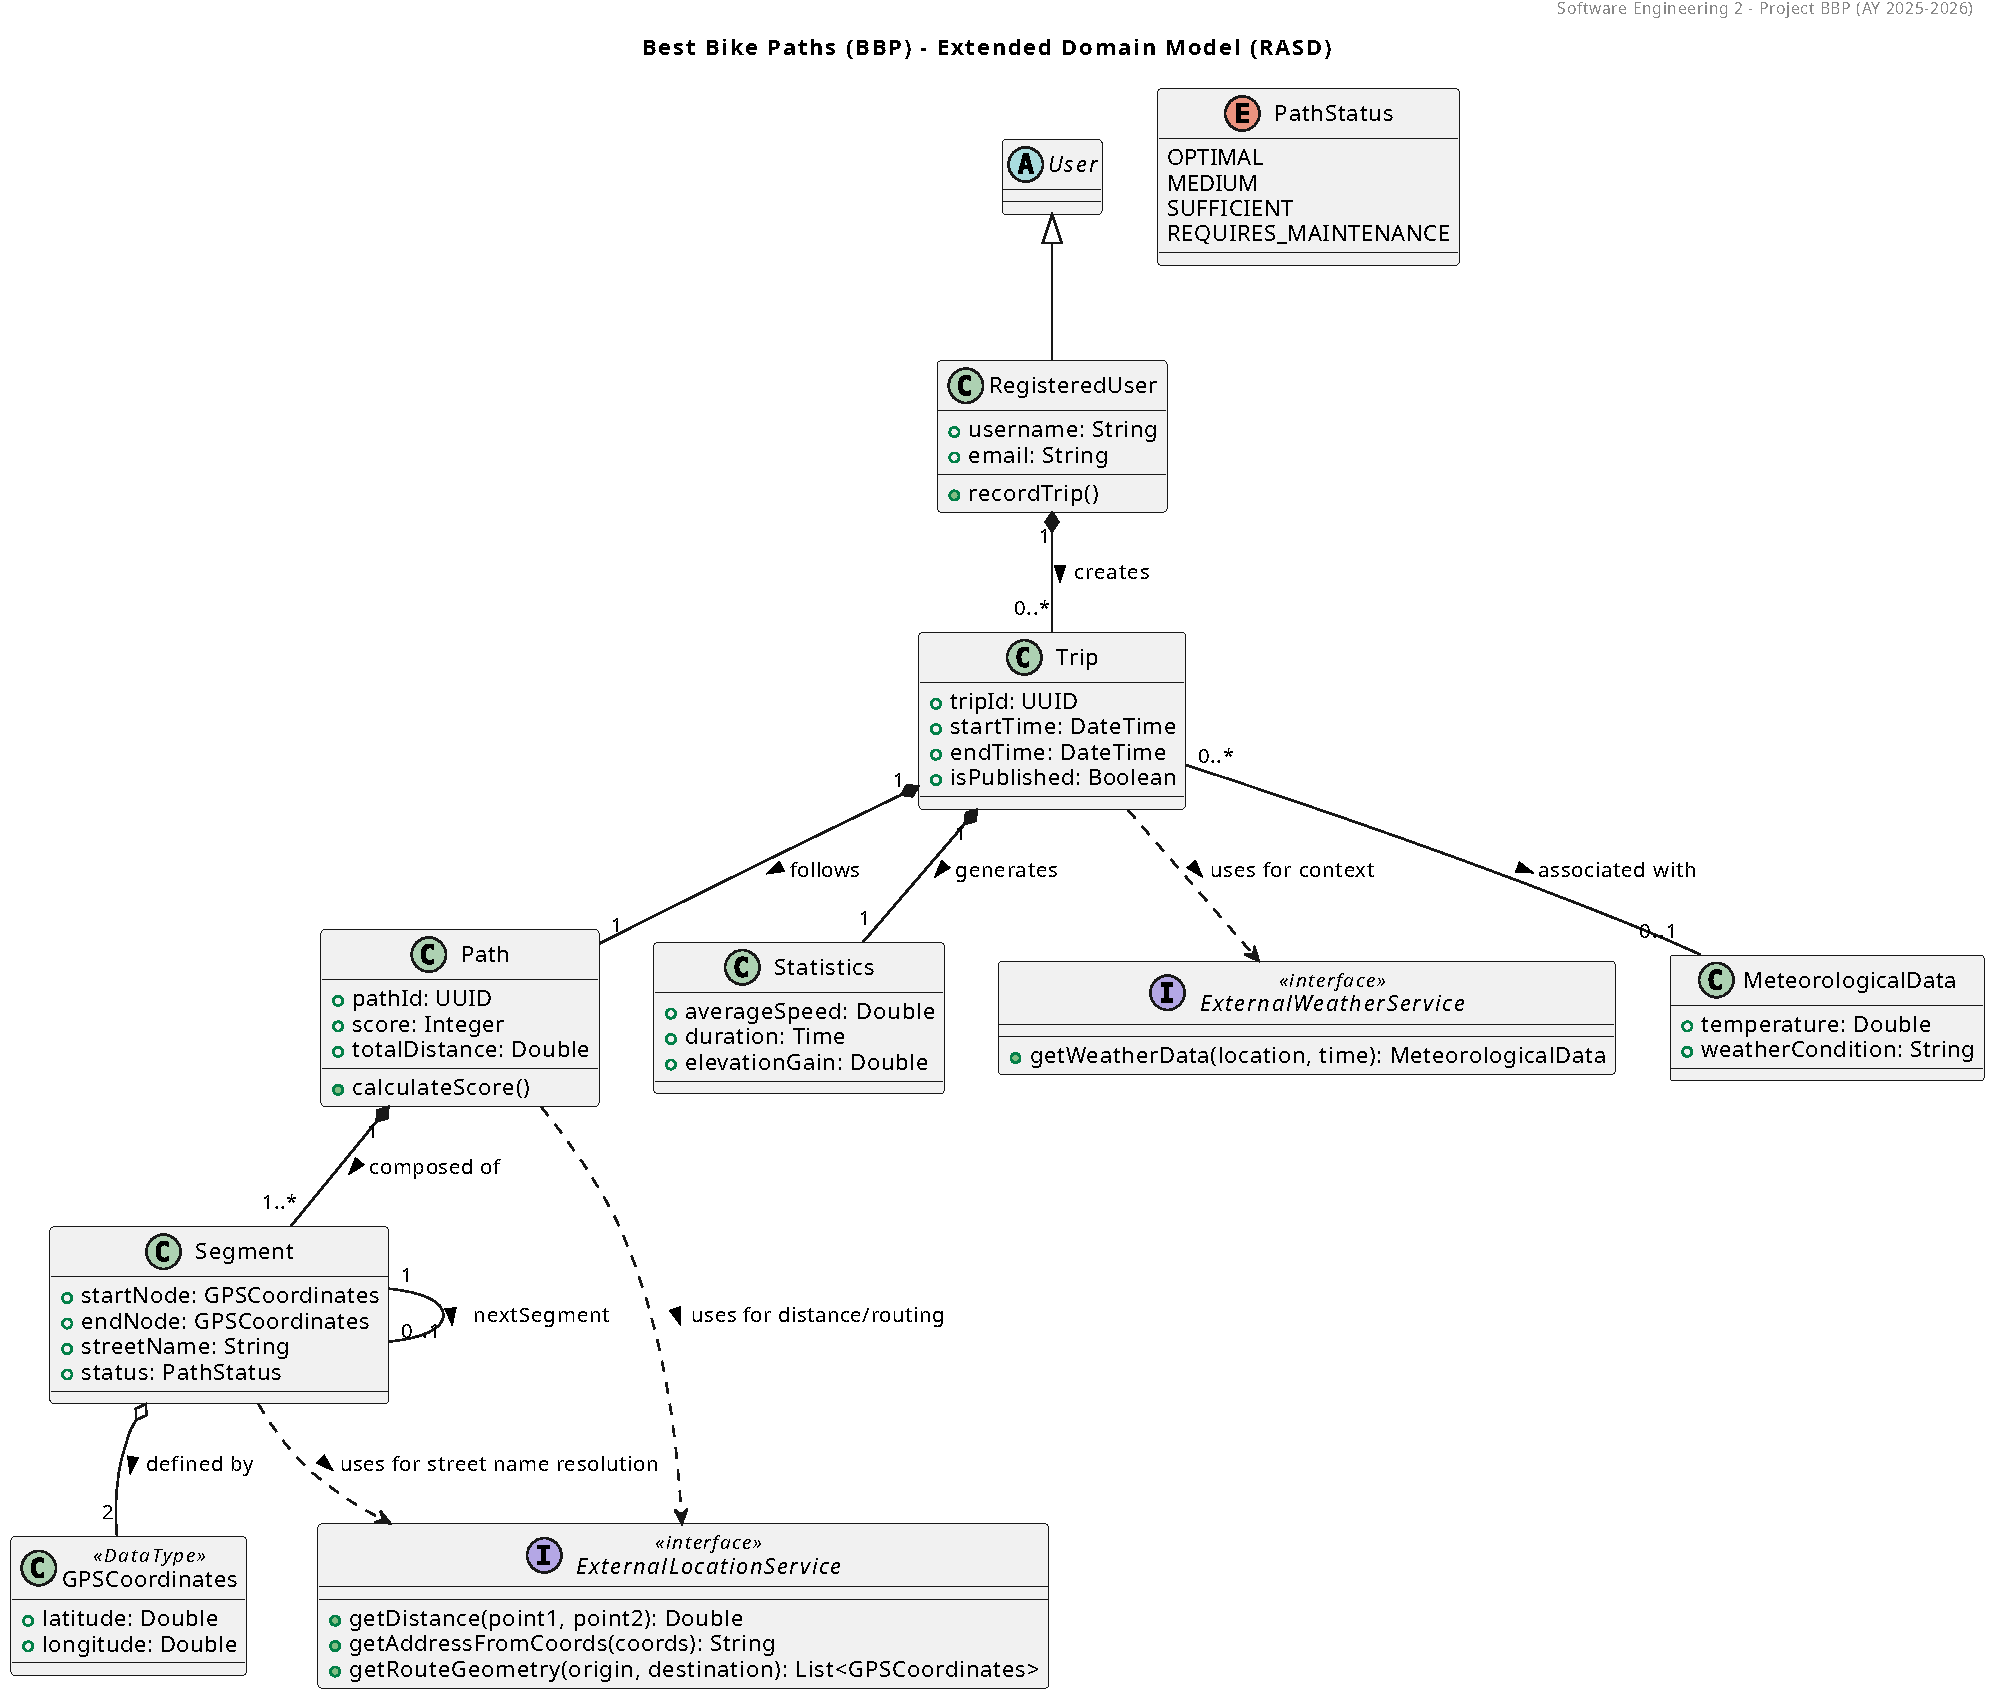
\includegraphics[width=\textwidth]{Images/class_diagram.pdf}
    \caption{Class diagram representing the main entities and their relationships in the BBP system.}
\end{figure}


\subsection{State diagrams}

\textbf{Login and Registration}
This diagram depicts the user authentication flow. The application defaults to Guest Mode, which allows limited access to map visualization and routing. To perform active tasks like trip recording or data reporting, the user must enter an \texttt{Authenticated Session}. The model details the transitions for logging in, signing up, and handling session termination.
\begin{figure}[H]
    \centering
    \includegraphics[width=\textwidth]{"state_diagrams/login.pdf"}
    \caption{State diagram of the trip recording process.}
\end{figure}

\textbf{Automated trip recording}
The state diagram depicts the trip lifecycle, originating in the \texttt{MonitoringSpeed} state where the system samples GPS data. The transition to \texttt{Recording} occurs either manually or automatically when a speed threshold is exceeded, actively collecting sensor data in \texttt{AcquiringData} or temporarily shifting to \texttt{Paused} when stationary. The process concludes in \texttt{AwaitingAction}, where the user reviews statistics and confirms anomalies before the trip is finally \texttt{Saved} or \texttt{Discarded}.
\begin{figure}[H]
    \centering
    \includegraphics[width=\textwidth]{"state_diagrams/trip recording lifecycle.pdf"}
    \caption{State diagram of the trip recording process.}
\end{figure}

\textbf{Manual trip recording}
This diagram models the workflow for manually logging a trip after it has been completed (``offline reporting''). Since no real-time GPS tracking is involved, the user first provides general metadata (Origin, Destination, Duration). Subsequently, the user reconstructs the route by inputting the sequence of streets traversed. The system then allows the user to annotate specific segments with details such as potholes or road status before finalizing the submission.
\begin{figure}[H]
    \centering
    \includegraphics[width=\textwidth]{"state_diagrams/manual.pdf"}
    \caption{State diagram of the manual trip registration process.}
\end{figure}

\textbf{Path data aggregation}
This diagram illustrates the backend logic for updating path attributes when new user data is submitted. The system first matches the recorded GPS trace against existing road segments in the database. It then compares the new report with historical data. If the new data confirms the existing status, the confidence score is boosted. If a conflict arises (e.g., a user reports a pothole on a previously ``Optimal'' path), the system applies a weighting algorithm based on data freshness to resolve the discrepancy and update the public score.
\begin{figure}[H]
    \centering
    \includegraphics[width=\textwidth]{"state_diagrams/matching.pdf"}
    \caption{State diagram of the path data aggregation process.}
\end{figure}

\textbf{Anomaly Detection and Validation}
This diagram illustrates the lifecycle of a road anomaly (e.g., a pothole) from detection to publication. Since sensor data can generate false positives, the system implements a validation step. Potential anomalies are first flagged internally as ``Candidates'' and presented to the user at the end of the trip for confirmation before being stored as valid data.











\section{Product functions}
\textbf{User Registration and Authentication:} Allows new users to create an account to access personalized features such as trip recording and data contribution. It handles secure login procedures and manages session states, ensuring that only authenticated users can modify the system's data.

\textbf{Guest Access Management:} Provides limited access to unregistered users (guests), allowing them to browse the map and search for bike paths without logging in. This function ensures that the public utility aspect of the system—viewing shared path information—is available to everyone.

\textbf{Account and Profile Management:} Enables registered users to manage their personal information and preferences. This includes viewing their stored data and managing their privacy settings regarding the publishable information they contribute to the community.

\textbf{Path Search and Visualization:} Allows users (both registered and guests) to specify an origin and a destination to retrieve available bike paths. It renders these paths on an interactive map, highlighting the most effective routes based on the system's scoring algorithm.

\textbf{Trip Recording (Automated and Manual):} Manages the acquisition of trip data. It supports a manual start/stop mechanism and an automated mode that "guesses" when the user is biking based on speed. It collects GPS coordinates for the route and sensor data (accelerometer/gyroscope) for anomaly detection.

\textbf{Path Status Reporting:} Provides an interface for users to manually insert data about street segments, such as maintenance status (e.g., "optimal," "requires maintenance") or specific obstacles. It also handles the user validation step required to confirm automatically detected anomalies like potholes.

\textbf{Trip History and Statistics:} Stores the details of completed trips for registered users, creating a personal log of cycling activities. It computes and displays key performance metrics for each trip, such as total distance covered and average speed.

\textbf{Meteorological Data Integration:} Connects to external weather services to retrieve environmental conditions (temperature, wind speed) for the specific time and location of a trip. It enriches the trip history with this context to help users analyze their performance relative to the weather.

\textbf{Path Scoring and Ranking:} Implements the logic to calculate a "score" for each path segment. This calculation considers the physical status of the road and its effectiveness in connecting the origin to the destination, ensuring the best paths are suggested first.

\textbf{Information Merging and Data Consistency:} Aggregates data received from multiple users regarding the same path segment. It applies specific rules to resolve conflicts—prioritizing data freshness and the number of confirming reports—to determine the current, most accurate status of a bike path.
\section{User charateristic}
The user population of the Best Bike Paths (BBP) system consists primarily of individuals who use bicycles for commuting, leisure, or sport. The user base is heterogeneous regarding age and technical skills, assuming only a basic familiarity with smartphone applications.

We identify two main categories of users:

\begin{itemize}
    \item \textbf{Registered Users}: This category represents the core user base of the application.
    \begin{itemize}
        \item \textit{Goals}: They use the system to track their cycling activities, store trip history, monitor performance statistics (e.g., speed, distance), and contribute to the community by reporting road conditions.
        \item \textit{Capabilities}: They have access to all system features, including data acquisition (Manual and Automated modes) and data visualization.
        \item \textit{Context}: They are willing to share their location data and sensor readings to assist the community and maintain a personal log of their rides.
    \end{itemize}

    \item \textbf{Unregistered Users (Guests)}: This category includes occasional users or those concerned with privacy who do not wish to create an account.
    \begin{itemize}
        \item \textit{Goals}: Their primary goal is to use the "passive" features of the system, specifically searching for bike paths and visualizing the best routes between an origin and a destination.
        \item \textit{Capabilities}: Their access is limited to the browsing and routing functionalities; they cannot record trips, save history, or contribute data to the system.
    \end{itemize}
\end{itemize}
\section{Assumptions, dependencies and constraints}

\subsection{Domain assumptions}
\begin{itemize}
    \item \textbf{GPS Accuracy:} It is assumed that the GPS sensors on users' mobile devices provide a level of accuracy sufficient to identify specific street segments, typically within a range of 5--10 meters.
    \item \textbf{Internet Connectivity:} Users are assumed to have access to a stable internet connection (WiFi or mobile data) at the end of their trips to allow the synchronization of recorded data with the BBP servers.
    \item \textbf{Map Service Reliability:} External map providers (e.g., Google Maps, OpenStreetMap) are assumed to provide up-to-date and accurate information regarding road networks, street names, and cycling-compatible paths.
    \item \textbf{User Honesty and Reliability:} It is assumed that registered users provide truthful information when manually inserting path status or confirming automated detections of obstacles like potholes.
    \item \textbf{Availability of External APIs:} External services for meteorological data and geocoding are assumed to be operational and reachable via standard protocols when the system needs to enrich trip data.
    \item \textbf{Device Sensor Functionality:} For automated data acquisition, it is assumed that the users' smartphones are equipped with functioning accelerometers and gyroscopes capable of detecting significant movement anomalies.
    \item \textbf{Path Decomposition:} Every bike path can be logically represented as a continuous sequence of segments, where each segment corresponds to a physical portion of the road network.
\end{itemize}